% Importado desde: 2026-03-28_Nielsen_Ninomiya_en_Weyl_y_Dirac_3p1.tex
\chapter{Derivacion Pedagogica: --- Nielsen--Ninomiya en el paso de Weyl a Dirac \(3+1\)}
\label{ch:nielsen-ninomiya-weyl-dirac-3p1}

\section{Objetivo}
Ya vimos tres piezas centrales del proyecto:
\begin{enumerate}[label=\arabic*.]
    \item una dinamica discreta tipo Weyl en \(3D\);
    \item el acoplamiento de dos sectores quirales para obtener Dirac;
    \item la estructura algebraica de rotaciones, boosts y matrices gamma.
\end{enumerate}

Ahora toca insertar dentro de ese hilo el obstaculo estructural mas serio del programa:
\begin{displayquote}
\textbf{en una red discreta traslacionalmente invariante, un nodo de Weyl aislado no aparece solo.}
\end{displayquote}

Este capitulo reescribe Nielsen--Ninomiya justo en el punto donde nos importa:
\begin{enumerate}[label=\arabic*.]
    \item construiremos un Hamiltoniano de red minimo tipo Weyl;
    \item localizaremos todos sus nodos en la zona de Brillouin;
    \item calcularemos la quiralidad de cada uno;
    \item veremos por que la suma total de quiralidades es cero;
    \item explicaremos que significa eso para el paso de Weyl a Dirac \(3+1\).
\end{enumerate}

\section{Por que el problema aparece justamente ahora}
En los capitulos anteriores trabajamos muchas veces cerca de un nodo y linealizamos. Ese procedimiento es correcto localmente, pero una red no vive solo cerca de un punto. Vive en toda la zona de Brillouin, que es compacta y periodica.

Esa periodicidad cambia por completo la historia global:
\begin{equation}
\bm{k}\sim \bm{k}+\bm{G},
\end{equation}
donde \(\bm{G}\) es un vector recíproco.

La consecuencia conceptual es fuerte:
\begin{displayquote}
\textbf{si un nodo Weyl actua como fuente topologica de curvatura de Berry, otro nodo debe actuar como sumidero para compensar en la zona de Brillouin completa.}
\end{displayquote}

Por eso Nielsen--Ninomiya no es un detalle tecnico lateral. Es la restriccion que nos dice cuantas quiralidades puede producir de verdad una red.

\begin{figure}[h!]
\centering
\begin{tikzpicture}[
    box/.style={draw, rounded corners, thick, align=center, minimum width=3.6cm, minimum height=1.3cm},
    arr/.style={-{Latex[length=3mm]}, thick}
]
\node[box, fill=blue!7] (a) at (0,0) {Analisis local\\cerca de un nodo};
\node[box, fill=green!7] (b) at (4.8,0) {Zona de Brillouin\\compacta};
\node[box, fill=yellow!10] (c) at (9.6,0) {Suma total de\\quiralidades = 0};
\node[box, fill=red!7] (d) at (14.4,0) {No hay un Weyl\\aislado};
\draw[arr] (a) -- (b);
\draw[arr] (b) -- (c);
\draw[arr] (c) -- (d);
\end{tikzpicture}
\caption{La logica global que impone Nielsen--Ninomiya.}
\end{figure}

\section{Un modelo de red minimo tipo Weyl}
\subsection{Hamiltoniano}
Tomamos el Hamiltoniano de Bloch mas simple que reproduce una estructura tipo Weyl:
\begin{equation}
H(\bm{k}) = \frac{v}{a}\left(
\sigma_x \sin k_x a +
\sigma_y \sin k_y a +
\sigma_z \sin k_z a
\right),
\label{c27:eq:naiveweyl}
\end{equation}
donde \(a\) es el espaciado de red y \(\bm{k}\) vive en la zona de Brillouin
\begin{equation}
-\frac{\pi}{a}\le k_i < \frac{\pi}{a}.
\end{equation}

Este modelo es exactamente el análogo tridimensional de la discretizacion ingenua del fermion de Dirac. Es local, traslacionalmente invariante y perfectamente periodico en el espacio recíproco.

\subsection{Espectro}
Como \(H(\bm{k})\) es de dos bandas, su espectro sale inmediatamente:
\begin{equation}
E(\bm{k})=
\pm \frac{v}{a}
\sqrt{
\sin^2(k_x a)+\sin^2(k_y a)+\sin^2(k_z a)
}.
\label{c27:eq:spec}
\end{equation}

Los nodos aparecen cuando la raiz se anula, es decir cuando
\begin{equation}
\sin(k_x a)=\sin(k_y a)=\sin(k_z a)=0.
\label{c27:eq:zeros}
\end{equation}

Dentro de la primera zona de Brillouin eso ocurre para
\begin{equation}
k_i \in \left\{0,\frac{\pi}{a}\right\}.
\end{equation}

Por tanto no aparece un solo nodo, sino
\begin{equation}
2^3 = 8
\end{equation}
nodos distintos.

\section{Donde estan los nodos}
Los ocho nodos se etiquetan por
\begin{equation}
\bm{k}^{(n_x n_y n_z)}=
\left(
\frac{n_x\pi}{a},
\frac{n_y\pi}{a},
\frac{n_z\pi}{a}
\right),
\qquad
n_i\in\{0,1\}.
\label{c27:eq:nodes}
\end{equation}

\begin{figure}[h!]
\centering
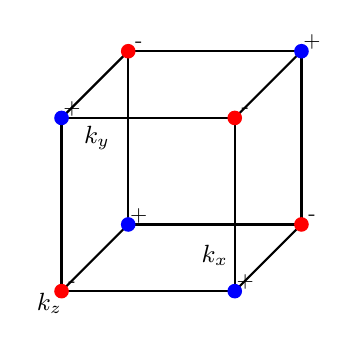
\begin{tikzpicture}[scale=2.2]
\draw[thick] (0,0,0) -- (1,0,0);
\draw[thick] (0,0,0) -- (0,1,0);
\draw[thick] (0,0,0) -- (0,0,1);
\draw[thick] (1,0,0) -- (1,1,0);
\draw[thick] (1,0,0) -- (1,0,1);
\draw[thick] (0,1,0) -- (1,1,0);
\draw[thick] (0,1,0) -- (0,1,1);
\draw[thick] (0,0,1) -- (1,0,1);
\draw[thick] (0,0,1) -- (0,1,1);
\draw[thick] (1,1,0) -- (1,1,1);
\draw[thick] (1,0,1) -- (1,1,1);
\draw[thick] (0,1,1) -- (1,1,1);

\foreach \x/\y/\z/\col/\lab in {
0/0/0/blue/{+},
1/0/0/red/{-},
0/1/0/red/{-},
0/0/1/red/{-},
1/1/0/blue/{+},
1/0/1/blue/{+},
0/1/1/blue/{+},
1/1/1/red/{-}}
{
    \fill[\col] (\x,\y,\z) circle (1.2pt);
    \node[scale=0.8] at (\x+0.08,\y+0.07,\z+0.05) {\lab};
}

\node at (0.5,-0.18,0) {\small \(k_x\)};
\node at (-0.18,0.5,0) {\small \(k_y\)};
\node at (0,0,1.18) {\small \(k_z\)};
\end{tikzpicture}
\caption{Esquema de los ocho nodos del modelo ingenuo en la zona de Brillouin. El signo indica la quiralidad que calcularemos enseguida.}
\end{figure}

\section{Linealizacion alrededor de cada nodo}
Sea
\begin{equation}
\bm{k}=\bm{k}^{(n_x n_y n_z)}+\bm{q},
\qquad
\abs{\bm{q}}\ll \frac{\pi}{a}.
\end{equation}
Entonces
\begin{equation}
\sin\!\left(\frac{n_i\pi}{a}a + q_i a\right)
=
\sin(n_i\pi + q_i a)
=
(-1)^{n_i}\sin(q_i a).
\end{equation}

Para \(qa\ll 1\),
\begin{equation}
\sin(q_i a)\simeq q_i a,
\end{equation}
de modo que el Hamiltoniano linealizado queda
\begin{equation}
H_{(n_x n_y n_z)}(\bm{q})
\simeq
v\left(
(-1)^{n_x}\sigma_x q_x +
(-1)^{n_y}\sigma_y q_y +
(-1)^{n_z}\sigma_z q_z
\right).
\label{c27:eq:linearized}
\end{equation}

Asi, cada nodo se comporta localmente como un Hamiltoniano de Weyl, pero con una matriz de velocidades
\begin{equation}
V^{(n)}=
v\,
\mathrm{diag}\!\left(
(-1)^{n_x},
(-1)^{n_y},
(-1)^{n_z}
\right).
\end{equation}

\section{Calculo de la quiralidad}
La quiralidad local de un nodo Weyl se define por el signo del determinante de su matriz de velocidades:
\begin{equation}
\chi_n = \mathrm{sign}\det V^{(n)}.
\label{c27:eq:chirdef}
\end{equation}

En nuestro caso,
\begin{equation}
\det V^{(n)}
=
v^3(-1)^{n_x+n_y+n_z},
\end{equation}
de manera que
\begin{equation}
\boxed{
\chi_n = (-1)^{n_x+n_y+n_z}.
}
\label{c27:eq:chirality}
\end{equation}

Esto significa:
\begin{enumerate}[label=\arabic*.]
    \item si \(n_x+n_y+n_z\) es par, la quiralidad es \(+1\);
    \item si \(n_x+n_y+n_z\) es impar, la quiralidad es \(-1\).
\end{enumerate}

La distribucion explicita queda en la tabla:

\begin{center}
\begin{tabular}{ccc c c}
\toprule
\(n_x\) & \(n_y\) & \(n_z\) & nodo & \(\chi\) \\
\midrule
0 & 0 & 0 & \((0,0,0)\) & \(+1\) \\
1 & 0 & 0 & \((\pi/a,0,0)\) & \(-1\) \\
0 & 1 & 0 & \((0,\pi/a,0)\) & \(-1\) \\
0 & 0 & 1 & \((0,0,\pi/a)\) & \(-1\) \\
1 & 1 & 0 & \((\pi/a,\pi/a,0)\) & \(+1\) \\
1 & 0 & 1 & \((\pi/a,0,\pi/a)\) & \(+1\) \\
0 & 1 & 1 & \((0,\pi/a,\pi/a)\) & \(+1\) \\
1 & 1 & 1 & \((\pi/a,\pi/a,\pi/a)\) & \(-1\) \\
\bottomrule
\end{tabular}
\end{center}

\section{La cancelacion global}
Sumando todas las quiralidades obtenemos
\begin{equation}
\sum_n \chi_n = 4 - 4 = 0.
\label{c27:eq:sumzero}
\end{equation}

Esta ecuacion es la version mas concreta del mensaje de Nielsen--Ninomiya para este modelo. La red no produce un solo Weyl de una mano, sino un conjunto completo cuya carga quiral total se anula.

\subsection{Lectura topologica}
Cada nodo Weyl puede pensarse como una fuente o sumidero de flujo de curvatura de Berry en el espacio recíproco:
\begin{enumerate}[label=\arabic*.]
    \item \(\chi=+1\): fuente;
    \item \(\chi=-1\): sumidero.
\end{enumerate}

Pero la zona de Brillouin es compacta. No hay \enquote{infinito} por donde se escape un flujo neto. Por eso la suma total debe cancelarse.

\begin{figure}[h!]
\centering
\begin{tikzpicture}[
    posnode/.style={circle, draw=blue!70!black, fill=blue!15, minimum size=8mm},
    negnode/.style={circle, draw=red!70!black, fill=red!15, minimum size=8mm},
    arr/.style={-{Latex[length=2.5mm]}, thick}
]
\node[posnode] (p1) at (0,1.8) {\(+\)};
\node[posnode] (p2) at (0,-1.8) {\(+\)};
\node[negnode] (n1) at (5,1.8) {\(-\)};
\node[negnode] (n2) at (5,-1.8) {\(-\)};

\draw[arr, blue!70!black] (p1) -- (2.1,1.8);
\draw[arr, blue!70!black] (p1) -- (1.6,0.9);
\draw[arr, blue!70!black] (p1) -- (1.6,2.7);
\draw[arr, blue!70!black] (p2) -- (2.1,-1.8);
\draw[arr, blue!70!black] (p2) -- (1.6,-0.9);
\draw[arr, blue!70!black] (p2) -- (1.6,-2.7);

\draw[arr, red!70!black] (2.9,1.8) -- (n1);
\draw[arr, red!70!black] (3.4,0.9) -- (n1);
\draw[arr, red!70!black] (3.4,2.7) -- (n1);
\draw[arr, red!70!black] (2.9,-1.8) -- (n2);
\draw[arr, red!70!black] (3.4,-0.9) -- (n2);
\draw[arr, red!70!black] (3.4,-2.7) -- (n2);
\end{tikzpicture}
\caption{Lectura intuitiva: las fuentes y sumideros deben compensarse globalmente.}
\end{figure}

\section{Que significa esto para nuestro paso Weyl \texorpdfstring{\(\to\)}{->} Dirac}
Ahora podemos reinterpretar mejor el capitulo donde construimos Dirac a partir de dos sectores Weyl.

\subsection{Lo que sigue siendo correcto}
El paso local
\begin{equation}
\text{Weyl izquierdo} + \text{Weyl derecho} + \text{masa}
\longrightarrow
\text{Dirac}
\end{equation}
es completamente correcto a nivel de teoria efectiva cerca de un par de nodos apropiado.

\subsection{Lo que cambia globalmente}
Pero en una red real no solemos tener solo \enquote{ese par}. Lo natural es que existan mas nodos, y la seleccion de un par concreto requiere una justificacion adicional:
\begin{enumerate}[label=\arabic*.]
    \item simetria;
    \item estructura de bandas;
    \item termino de Wilson u otra deformacion;
    \item mecanismos topologicos o cristalinos mas finos.
\end{enumerate}

En otras palabras:
\begin{displayquote}
\textbf{el bloque local Weyl \(\to\) Dirac no desaparece, pero Nielsen--Ninomiya nos obliga a insertarlo dentro de una arquitectura global mas amplia.}
\end{displayquote}

\section{Como se conecta con el modelo discreto del capitulo previo}
En el capitulo \enquote{Weyl \(3D\) a Dirac \(3+1\)} trabajamos con una dinamica efectiva construida como producto de pasos unitarios en tres direcciones. Esa construccion es buena como aproximacion local cerca de un nodo.

Lo que Nielsen--Ninomiya añade es esta advertencia:
\begin{equation}
\text{localmente: un Weyl},\qquad
\text{globalmente en la red: varios Weyl con quiralidad total nula}.
\end{equation}

Esto aclara muy bien el estatus de lo ya hecho:
\begin{enumerate}[label=\arabic*.]
    \item la derivacion local era correcta;
    \item pero no agotaba la informacion global de la zona de Brillouin;
    \item para una teoria discreta completa, la contabilidad de nodos es obligatoria.
\end{enumerate}

\section{La salida pedagogica mas simple: termino de Wilson}
La manera mas clasica de romper la degeneracion ingenua es agregar un termino que se anule cerca del nodo deseado pero gappee a los dobladores lejanos. En el lenguaje de red, la forma prototipica es
\begin{equation}
H_W(\bm{k}) =
\frac{r}{a}
\sum_{i=1}^3
\left(1-\cos k_i a\right)\sigma_0,
\end{equation}
o, para un problema Dirac de cuatro bandas, una version análoga acoplada a la matriz de masa.

La idea pedagogica no es memorizar la forma exacta, sino entender lo que hace:
\begin{enumerate}[label=\arabic*.]
    \item cerca de \(k_i=0\), \(1-\cos k_i a \sim (k_i a)^2/2\), asi que afecta poco al nodo central;
    \item cerca de \(k_i=\pi/a\), \(1-\cos k_i a = 2\), asi que cambia mucho la energia de los dobladores.
\end{enumerate}

Asi, el termino de Wilson no destruye la descripcion de baja energia deseada, pero si reorganiza fuertemente la estructura global de nodos.

\begin{figure}[h!]
\centering
\begin{tikzpicture}[
    box/.style={draw, rounded corners, thick, align=center, minimum width=3.9cm, minimum height=1.4cm},
    arr/.style={-{Latex[length=3mm]}, thick}
]
\node[box, fill=blue!7] (a) at (0,0) {modelo ingenuo\\muchos nodos};
\node[box, fill=yellow!10] (b) at (5.1,0) {agregar termino\\de Wilson};
\node[box, fill=green!7] (c) at (10.2,0) {gappear dobladores\\lejanos};
\node[box, fill=red!7] (d) at (15.3,0) {controlar mejor el\\sector efectivo};
\draw[arr] (a) -- (b);
\draw[arr] (b) -- (c);
\draw[arr] (c) -- (d);
\end{tikzpicture}
\caption{La funcion conceptual del termino de Wilson.}
\end{figure}

\section{Lecciones para el programa de investigacion}
Este capitulo deja cinco mensajes practicos.

\subsection*{Mensaje 1}
Un nodo Weyl aislado no es la situacion generica de una red discreta regular.

\subsection*{Mensaje 2}
La quiralidad es una propiedad local, pero su suma total esta restringida globalmente por la compactificacion de la zona de Brillouin.

\subsection*{Mensaje 3}
El paso local de dos sectores Weyl a un fermion de Dirac sigue siendo correcto, pero debe verse como seleccion de un subsector efectivo, no como descripcion completa de toda la red.

\subsection*{Mensaje 4}
Toda ambicion de reconstruir Dirac \(3+1\) desde una estructura discreta exige controlar no solo un nodo, sino la familia completa de dobladores.

\subsection*{Mensaje 5}
La siguiente pregunta natural ya no es solo algebraica, sino de diseño de modelo:
\begin{displayquote}
\textbf{que dinamica discreta en \(3D\) permite aislar o controlar el subsector que mejor aproxima la estructura relativista efectiva deseada?}
\end{displayquote}

\section{Mapa del siguiente paso}
Despues de este capitulo, el hilo mas natural es:
\begin{enumerate}[label=\arabic*.]
    \item tomar una dinamica discreta concreta en \(3D\);
    \item identificar sus nodos y su contabilidad quiral;
    \item estudiar que terminos o simetrias permiten seleccionar un subsector efectivo util;
    \item volver entonces a la pregunta de si, en ese subsector, emergen no solo las gamma sino tambien una estructura razonable de generadores efectivos.
\end{enumerate}

\section{Resumen final}
El mensaje central de Nielsen--Ninomiya, traducido al punto donde estamos del proyecto, es muy claro. Una red discreta local y periodica puede producir conos de Weyl, pero no uno solo de manera aislada. En el ejemplo minimo
\[
H(\bm{k})=\frac{v}{a}\sum_i \sigma_i \sin(k_i a),
\]
aparecen ocho nodos en la zona de Brillouin, y sus quiralidades se distribuyen de tal modo que la suma total es cero.

Eso no destruye la idea del proyecto, pero la vuelve mas precisa. El paso local \enquote{Weyl \(\to\) Dirac} sigue siendo correcto, aunque ahora entendemos que cualquier realizacion discreta completa debe justificar por que cierto par de sectores es el fisicamente relevante y como se controlan los demas. Dicho de otro modo: Nielsen--Ninomiya no cancela el programa; le impone disciplina estructural.
